\title{BT5110 Data Management and Warehousing}

\subtitle{Tutorial 2: Simple and Algebra\"{\i}c Queries}

\author{Mark Meng Huasong}

\institute[National University of Singapore] % (optional, but mostly needed)
{
	School of Computing\\
	National University of Singapore
}

\titlegraphic{
	
\includegraphics[width=2cm]{nus-logo}
}

\date{30 Aug - 3 Sep, 2021}

\begin{frame}
	\titlepage
\end{frame}

\begin{frame}[fragile]{Quick Recap: End of Last Tutorial}
	\begin{figure}
		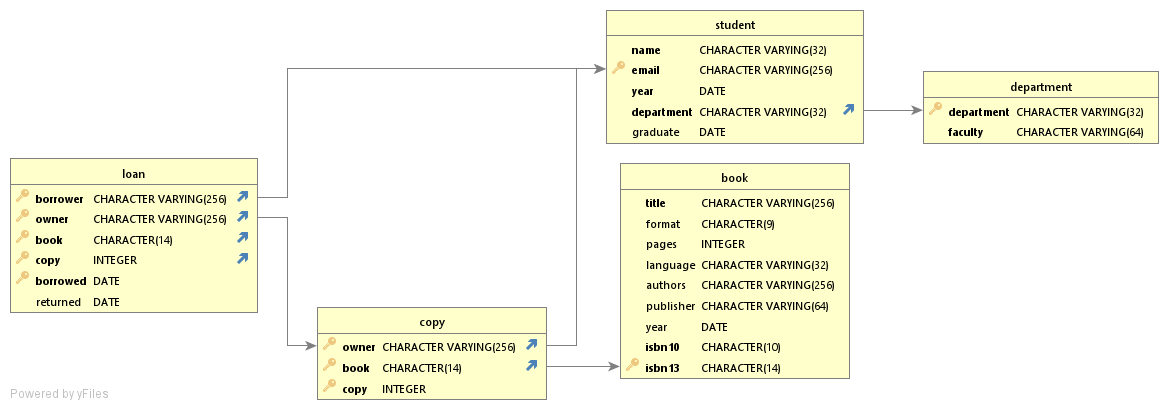
\includegraphics[width=1\textwidth]{t1/images/t1-end.png}
	\end{figure}
	(plotted by DbVisualizer)
\end{frame}

\section*{Question 1 Simple Queries}

\begin{frame}[fragile]{Question 1 (a-c)}
	(a) Print the different departments.\\ \vspace{5pt}
	(b) Print the different departments in which students are enrolled. \\ \vspace{5pt}
	(c) Let us check the integrity of the data. Print the emails of the students who borrowed or lent a copy of a book before they joined the university. There should not be any. Use a simple query.  
\end{frame}

\begin{frame}[fragile]{Solution 1 (a, b)}

\begin{lstlisting}		
SELECT d.department FROM department d;
\end{lstlisting}

Notice that the query does not require \texttt{DISTINCT} to eliminate duplicates. Duplicates are guaranteed not to occur because \texttt{department} is the \texttt{PRIMARY KEY} of the table \texttt{department}

\begin{lstlisting}
SELECT DISTINCT s.department FROM student s;
\end{lstlisting}

There could be departments in which no student is enrolled. This is the case of the department of \texttt{Undecidable Computations}.  We need to look into the \texttt{student} table.

\end{frame}

\begin{frame}[fragile]{Solution 1 (a, b) Cont.}

\begin{alertblock}{Notice}
	The outputs of these two queries have the same contents but with different orders.
\end{alertblock}\vspace{10pt}

	\begin{columns}
		\column{0.45\textwidth}
		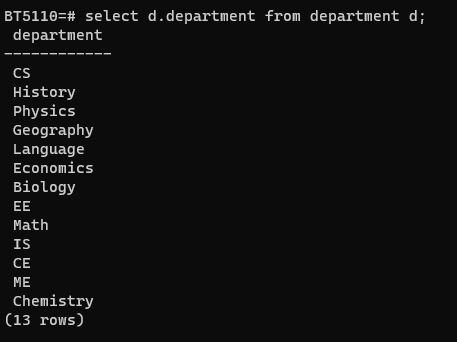
\includegraphics[width=\textwidth]{t2/images/t2-1a.png}
		
		\column{0.5\textwidth}
		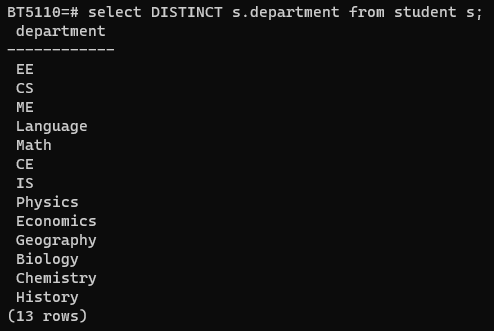
\includegraphics[width=\textwidth]{t2/images/t2-1b.png}
	\end{columns}
	
\end{frame}

\begin{frame}[fragile]{Solution 1 (c)}
(c) Let us check the integrity of the data. Print the emails of the students who borrowed or lent a copy of a book before they joined the university. There should not be any. Use a simple query.\\\vspace{10pt}

\begin{lstlisting}
SELECT DISTINCT s.email FROM loan l, student s 
WHERE (s.email = l.borrower AND l.borrowed < s.year) 
	OR (s.email = l.owner AND l.borrowed < s.year);
\end{lstlisting}
\end{frame}


\begin{frame}[fragile]{Question 1 (d)}

For each copy that has been borrowed and returned, print the \textbf{duration} of the loan. Order the results in \textbf{ascending} order of the ISBN13 and \textbf{descending} order of duration.  
\end{frame}

\begin{frame}[fragile]{Solution 1 (d)}

	\begin{lstlisting}
		SELECT book, returned - borrowed + 1 AS duration 
		FROM loan
		WHERE NOT (returned ISNULL)
		ORDER BY book ASC, duration DESC;
	\end{lstlisting}

\begin{alertblock}{Notice}
\texttt{ASC} is the default, but it is strongly recommended to indicate it for clarity.
\end{alertblock}	

\textbf{Result}: \textcolor{red}{4871} rows are returned ($\neq$ number of rows in table \texttt{loan}).\\\vspace{10pt}
\textcolor{orange}{Is this result correct?}
	
\end{frame}

\begin{frame}[fragile]{Solution 1 (d) Cont.}
	
Notice that the duration can be null if the book has not been returned yet. For a complete answer, you need to calculate the duration until a specific date (e.g., December 31, 2010) to include the books that have not been returned yet. \vspace{10pt}
	
\begin{lstlisting}
SELECT book, ((CASE	WHEN returned ISNULL 
		THEN '2010-12-31'
		ELSE returned END) - borrowed + 1) AS duration 
	FROM loan
	ORDER BY book ASC, duration ASC;
\end{lstlisting}
\vspace{10pt}
 
\textbf{Result}: \textcolor{red}{4976} rows are returned (= number of rows in table \texttt{loan})
\end{frame}


\begin{frame}[fragile]{Question 1 (e)}

For each loan of a book published by Wiley that has not been returned, print the title of the book, the name and faculty of the owner and the name and faculty of the borrower. Use \textbf{CROSS JOIN}.

\begin{figure}
	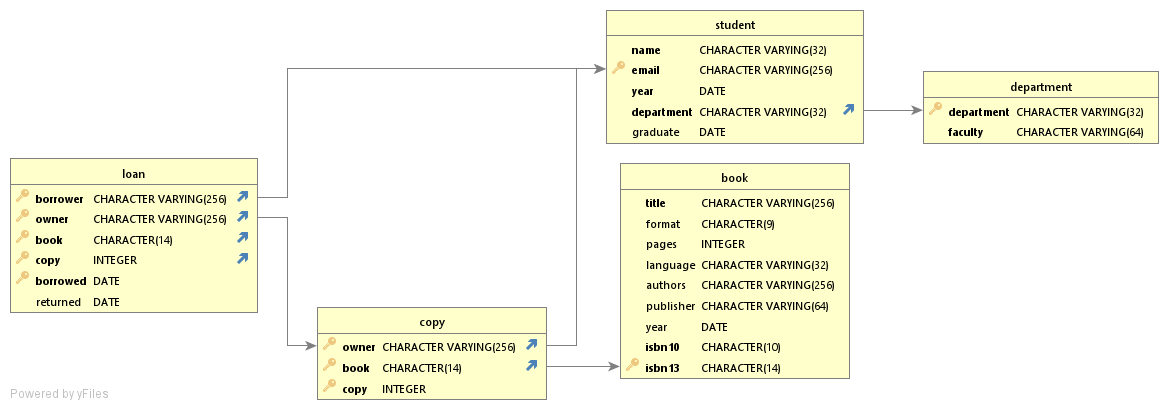
\includegraphics[width=0.9\textwidth]{t1/images/t1-end.png}
\end{figure}

\textcolor{orange}{Which table(s) is needed to be included in this query? how many instances of those tables are needed (e.g., how many students/departments are involved in per query result)?}
\end{frame}


\begin{frame}[fragile]{Solution 1 (e)}

We join primary keys and foreign keys to stitch tables together properly. 
	
	\begin{lstlisting}
		SELECT b.title, 
		s1.name AS ownername, 
		d1.faculty AS ownerFaculty, 
		s2.name AS borrowername, 
		d2.faculty AS  borrowerfaculty
		FROM loan l, book b,  copy c, 
		student s1, student s2, 
		department d1, department d2
		WHERE l.book=b.ISBN13
		AND c.book = l.book 
		AND c.copy = l.copy 
		AND c.owner = l.owner
		AND l.owner = s1.email
		AND l.borrower = s2.email
		AND s1.department = d1.department
		AND s2.department = d2.department
		AND b.publisher ='Wiley'
		AND l.returned ISNULL;
	\end{lstlisting}
	
	You can omit the table \texttt{copy}  and the \texttt{copy} column since the existence of the corresponding rows and values is guaranteed by design and by the foreign and primary key constraints.
	
	\begin{lstlisting}
		SELECT b.title, 
		s1.name AS ownername, 
		d1.faculty AS ownerFaculty, 
		s2.name AS borrowername, 
		d2.faculty AS  borrowerfaculty
		FROM loan l, book b,  
		student s1, student s2, 
		department d1, department d2
		WHERE l.book=b.ISBN13
		AND l.owner = s1.email
		AND l.borrower = s2.email
		AND s1.department = d1.department
		AND s2.department = d2.department
		AND b.publisher ='Wiley'
		AND l.returned ISNULL;
	\end{lstlisting}

\end{frame}

\section*{Question 2: Algebraic Queries}

\begin{frame}[fragile]{Question 2 (a)}
For each loan of a book published by Wiley that has not been returned, print the title of the book, the name and faculty of the owner and the name and faculty of the borrower. Use \textbf{INNER JOIN}.
\end{frame}

\begin{frame}[fragile]{Solution 2 (a)}
\begin{lstlisting}
	SELECT b.title, 
	s1.name AS ownername, 
	d1.faculty AS ownerFaculty, 
	s2.name AS borrowername, 
	d2.faculty AS  borrowerfaculty
	FROM loan l 
	INNER JOIN book b ON l.book=b.ISBN13
	INNER JOIN student s1 ON l.owner = s1.email
	INNER JOIN student s2 ON l.borrower = s2.email
	INNER JOIN department d1 ON s1.department = d1.department
	INNER JOIN department d2 ON s2.department = d2.department
	WHERE  b.publisher ='Wiley'
	AND l.returned ISNULL;
\end{lstlisting} 
\end{frame}

\begin{frame}[fragile]{Question 2 (b)}
Print the emails of the different students who borrowed or lent a copy of a book on the day that they joined the university. Use an algebra\"{\i}c query.
\end{frame}

\begin{frame}[fragile]{Solution 2 (b)}

\begin{lstlisting}
	SELECT  s.email 
	FROM loan l, student s 
	WHERE s.email = l.borrower AND l.borrowed = s.year
	UNION
	SELECT  s.email 
	FROM loan l, student s 
	WHERE s.email = l.owner AND l.borrowed = s.year;
\end{lstlisting}


\texttt{DISTINCT} is not needed because \texttt{UNION}  eliminates duplicates (so do \texttt{INTERSECT}, \texttt{EXCEPT} and \texttt{MINUS}). 

The corresponding simple query is generally preferable.

\begin{lstlisting}
	SELECT DISTINCT s.email 
	FROM loan l,  student s 
	WHERE (s.email = l.borrower OR s.email = l.owner) 
	AND l.borrowed = s.year;
\end{lstlisting}

The simple query requires an explicit \texttt{DISTINCT}.	
\end{frame}

\begin{frame}[fragile]{Question 2 (c)}
Print the emails of the different students who borrowed and lent a copy of a book on the day that they joined the university. Use an algebra\"{\i}c query.
\end{frame}

\begin{frame}[fragile]{Solution 2 (c)}
\begin{lstlisting}
	SELECT  s.email 
	FROM loan l, student s 
	WHERE s.email = l.borrower AND l.borrowed = s.year
	INTERSECT
	SELECT  s.email 
	FROM loan l, student s 
	WHERE s.email = l.owner AND l.borrowed = s.year;
\end{lstlisting}


Note that the corresponding simple query is more complicated. It needs two \texttt{loan} tables.

\begin{lstlisting}
	SELECT DISTINCT s.email 
	FROM loan l1, loan l2, student s 
	WHERE s.email = l1.borrower AND l1.borrowed = s.year 
	AND s.email = l2.owner AND l2.borrowed = s.year;
\end{lstlisting}
\end{frame}

\begin{frame}[fragile]{Question 2 (d)}
Print the emails of the students who borrowed but did not lend a copy of a book on the day that they joined the university. Use an algebra\"{\i}c query.
\end{frame}

\begin{frame}[fragile]{Solution 2 (d)}
\begin{lstlisting}
	SELECT  s.email 
	FROM loan l, student s 
	WHERE s.email = l.borrower AND l.borrowed = s.year
	EXCEPT
	SELECT  s.email 
	FROM loan l, student s 
	WHERE s.email = l.owner AND l.borrowed = s.year;
\end{lstlisting}

There is no corresponding simple query. We would need to use nested or aggregate queries for this type of questions.
\end{frame}

\begin{frame}[fragile]{Question \& Solution 2 (e)}
Print the ISBN13 of the books that have never been borrowed. Use an algebra\"{\i}c query.

\textbf{Solution}:
\begin{lstlisting}
	SELECT  b.ISBN13 
	FROM book b
	EXCEPT
	SELECT  l.book 
	FROM loan l
\end{lstlisting}

or, using an \textit{OUTER JOIN}, which introduces NULL values,

\begin{lstlisting}
	SELECT  b.ISBN13 
	FROM book b LEFT OUTER JOIN loan l ON b.isbn13 = l.book
	WHERE l.book ISNULL;
\end{lstlisting}

There is no corresponding simple query. We would need to use nested or aggregate queries for this type of questions.

\end{frame}

\begin{frame}{}
\centering  
For any further question, please feel free to email me:\vspace{10pt}

huasong.meng@u.nus.edu \vspace{20pt}

See you next week!
\end{frame}